
\chapter{\LaTeX{} Standards for LBNF/DUNE }
\label{ch:latex-stds}

This chapter provides guidelines on sectioning,  inserting figures, tables and references, and formatting numbers and units according to the \LaTeX{} configuration we have set up for LBNF/DUNE documents.

Typically the start of your chapter will be an introduction to or overview of the chapter itself. Recommendation: write the chapter first, then go back and write the introduction to it. It's more likely to be coherent!

%%%%%%%%%%%%%%%%%%%%%%%%%%%%%%%%%%%%%%%%%%%%%%%%%%%%%%%%%%%%%%%%%%%%
\section{Sectioning}
\label{sec:sectioning}

Most documents get subdivided into chapters (for larger documents) and/or sections and subsections. Please subdivide according to these standards:

\begin{itemize}
\item A subdivision of a larger portion should have content that relates to some aspect of the larger portion. 
\item  If you create one subdivision, create at least one more. Otherwise, the topic of your one subdivision is (by definition) the same as that of the larger portion.
\item In your \LaTeX{} source, add lines of percent signs (comments) to make it easy to find where sections begin and end, as illustrated in the source for this file. (This really helps the editor!)
\end{itemize}

\begin{verbatim}
%%%%%%%%%%%%%%%%%%%%%%%%%%%%%%%%%%%%%%%%%%%%%%%%%%%%%%%%%%%%%%%%%%%%
\end{verbatim}

The following sectioning macros are available, ordered from bigger to smaller:

\begin{verbatim}
\chapter{A Chapter}
\section{A Section}
\subsection{A Sub Section}
\subsubsection{A Sub Sub Section}
\end{verbatim}

Two sub's is all you get.  
Consult with the technical editors if you feel finer grained
sectioning is required.
Starting from \verb|\subsection|, this produces the following:

%%%%%%%%%%%%%%%%%%%%%%%%%%%%%%%%%%%%%
\subsection{A Sub Section}
\label{sec:sub}

This is a subsection.

%%%%%%%%%%%%%%%%%%%
\subsubsection{A Sub Sub Section}
\label{sec:subsub}

This is a subsubsection.

%%%%%%%%%%%%%%%%%%%
\subsubsection{A second Sub Sub Section}
\label{sec:subsub2}

Remember, if you have one, you need at least one more.

%%%%%%%%%%%%%%%%%%%%%%%%%%%%%%%%%%%%%
\subsection{A second Sub Section}
\label{sec:sub2}

Ditto.

%%%%%%%%%%%%%%%%%%%%%%%%%%%%%%%%%%%%%%%%%%%%%%%%%%%%%%%%%%%%%%%%%%%%
\section{Including Figures}
\label{sec:figures}

Instead of using the usual \texttt{figure} environment, please use the custom \texttt{cdrfigure}
environment in order to provide for a consistent presentation.
The environment is called with one optional and two required
arguments:

\begin{enumerate}
\item An initial, optional short caption to appear in the List Of Figures (LoF), in square brackets. This caption only needs to
identify the figure uniquely, it does not need to describe it fully.
\item A (required) label for referencing (do not prepend \texttt{fig:} to the label text --  \LaTeX{} will do that automatically). No spaces are allowed in the label. Curly brackets. It is helpful to have this label match the filename of the figure. 
\item The (required) full caption. Curly brackets, again.
\end{enumerate}

Usually the figure contains a graphic via an \texttt{includegraphics} statement.
The filename is assumed relative to a \texttt{graphicspath} as
mentioned in Section~\ref{ssec:files-pdunesp-tdr} and as such, please (a) put the file in the right place and (b) don't
 specify any directory parts in its name.
The file's extension may be omitted. Provide an image credit if appropriate. The entry looks like this:

\begin{verbatim}
    \begin{cdrfigure}[optional caption for LoF]{required-label}
     {required full caption (Credit: xyz)}
    \includegraphics[width=0.8\textwidth]{image-filename}
    \end{cdrfigure}
\end{verbatim}



\begin{cdrfigure}[An aerial photograph of Fermilab]{aerial}{An aerial photograph of Fermilab
    showing Wilson Hall and surrounding accelerator rings (Photo: Fermilab
    Visual Media Services)}
  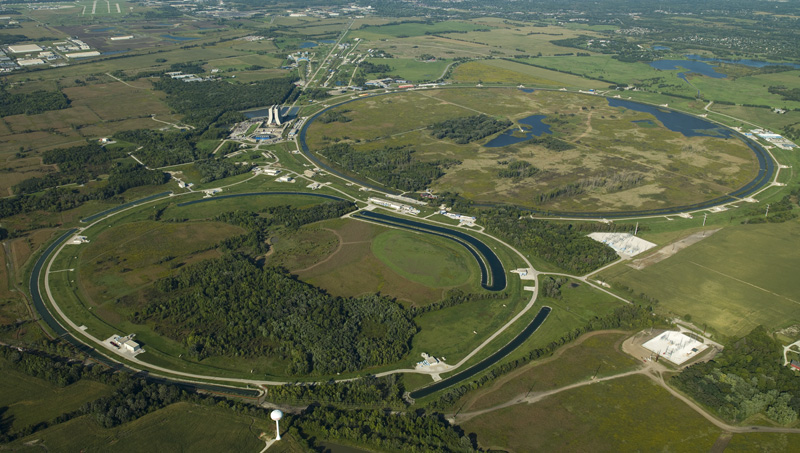
\includegraphics[width=0.8\textwidth]{fermilab-aerial.jpg}
\end{cdrfigure}


An example can be seen in Figure~\ref{fig:aerial}, which is created
with the \LaTeX{} shown in Figure~\ref{fig:aerial-latex}.  Notice that in the reference to the figures, we need to prepend \texttt{fig:} to the label. (See Section~\ref{sec:intra-doc-ref}.)

\begin{cdrfigure}[]{aerial-latex}{\LaTeX{} source showing how to include Figure~\ref{fig:aerial} and how to refer to it in the text}
\begin{verbatim}
    \begin{cdrfigure}[An aerial photograph of Fermilab]{aerial}
       {An aerial photograph of Fermilab showing Wilson Hall and 
       surrounding accelerator rings (Photo: Fermilab Visual Media Services)}
      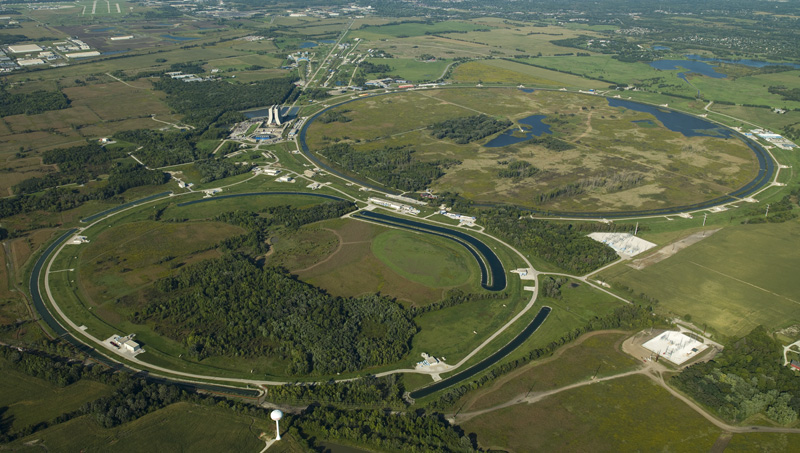
\includegraphics[width=0.8\textwidth]{fermilab-aerial.jpg}
      
      See Figure~\ref{fig:aerial}...
    \end{cdrfigure}
\end{verbatim}
\end{cdrfigure}

See Section~\ref{sec:figure-format} for guidelines on the graphics files themselves.

\FloatBarrier

%%%%%%%%%%%%%%%%%%%%%%%%%%%%%%%%%%%%%%%%%%%%%%%%%%%%%%%%%%%%%%%%%%%%
\section{Tables}
\label{sec:tables}

Like figures, we use a special environment, \texttt{cdrtable} for
tables to achieve a degree of consistency.
This is instead of the usual double \texttt{table} + \texttt{tabular} environments.
The \texttt{cdrtable} environment takes one optional and three
required arguments:

\begin{enumerate}
\item An initial, optional short caption for the List of Tables (LoT). Square brackets.
\item The tabular column specification. Curly brackets for the last three.
\item A label for referencing (it will have \texttt{tab:} prepended automatically)
\item The full caption.
\end{enumerate}

Inside the actual contents of the table you are required to provide an
initial row containing the headings for the table's rows followed by a
\texttt{toprowrule} macro.
Following every regular row (except the last) you should include a
\texttt{colline} macro.
Both of these take the place of the usual \texttt{hline}.

\begin{cdrtable}[The LoT caption]{cc}{example}
{This is a sample table.}
  Rows & Counts \\ \toprowrule
  Row 1 & First \\ \colhline
  Row 2 & Second \\ \colhline
  Row 3 & Third \\ 
\end{cdrtable}

\noindent Table~\ref{tab:example} is thus made like (arguments can span lines):

\begin{verbatim}
\begin{cdrtable}[The LoT caption]{cc}{example}
{This is an example table.}
  Rows & Counts \\ \toprowrule
  Row 1 & First \\ \colhline
  Row 2 & Second \\ \colhline
  Row 3 & Third \\ 
\end{cdrtable}

This is how you would make a reference to Table~\ref{tab:example}... 
\end{verbatim}

Table~\ref{tab:pdecay} shows a more complex example.
See the source for how it is written.
Note that special column specifications are used.

\begin{cdrtable}[Efficiencies and background rates for nucleon decay
  modes]{$L^c^c^c^c}{pdecay}{Efficiencies and background rates for
    nucleon decay channels of interest for a large underground LArTPC,
    and comparison with water Cherenkov detector capabilities} %$
  Decay Mode & \multicolumn{2}{^c}{Water Cherenkov} & 
\multicolumn{2}{^c}{Liquid Argon TPC} \\
\rowtitlestyle              % ``\rowstyletitle'' is needed here to bold the 2nd row of header text.
& Efficiency & Background & Efficiency & Background \\ \toprowrule
$p \rightarrow K^+ \overline{\nu}$ & 19\% & 4 & 97\% & 1 \\ \colhline
$p \rightarrow K^0 \mu^+$ & 10\% & 8 & 47\% & $<2 $ \\ \colhline
$p \rightarrow K^+ \mu^- \pi^+$ & & & 97\% & 1 \\ \colhline
$n \rightarrow K^+ e^- $ & 10\% & 3 & 96\% & $<2$ \\ \colhline
$n \rightarrow e^+\pi^-$ & 19\% & 2 & 44\% & 0.8 \\
\end{cdrtable}

\FloatBarrier



%%%%%%%%%%%%%%%%%%%%%%%%%%%%%%%%%%%%%%%%%%%%%%%%%%%%%%%%%%%%%%%%%%%%
\section{Labels and Intra-document References}
\label{sec:intra-doc-ref}

Assume that any chapter, section or important sub-, subsub- section
or any figure or table environment may need to be referenced
elsewhere in the text. 

Just below a chapter and any significant section heading a
\verb|\mylabel| should be added so it can be referenced. Use the defined label in a \verb|\ref{mylabel}| in order to make reference
to the chapter, section, figure, etc.

For example:

\begin{verbatim}
\chapter{A Chapter}
\label{ch:a-chapter}

\section{A Section}
\label{sec:a-section}

\subsection{A Sub Section}
\label{sec:a-subsection}

... as described in Chapter~\ref{ch:some-chapter} ... 
or Section~\ref{sec:a-section} ... 
or Section~\ref{sec:a-subsection} ...

\end{verbatim}


When you reference a chapter, section, subsection, figure, table,
etc., capitalize the word ``Chapter'' or whatever it is, e.g., ``as
shown in Section~\ref{sec:plots}.''
Use the word ``Section'' even if it's a subsection or subsubsection,
and use the tilde sign to keep the number on the same line as the word
that precedes it.

For figures, the reference needs to include ``fig:'' before the label name defined in the \verb|\cdrfigure| environment, as mentioned in Section~\ref{sec:figures}; for tables, ``tab:'' must be prepended to the label name (see Section~\ref{sec:tables}).


%%%%%%%%%%%%%%%%%%%%%%%%%%%%%%%%%%%%%%%%%%%%%%%%%%%%%%%%%%%%%%%%%%%%
\section{Citations and the Bibliography}

%%%%%%%%%%%%%%%%%%%%%%%%%%%%%%%%%%%%
\subsection{The File Containing the Citations}

The \texttt{citedb.bib} file is in BibTex format  (note that this filename may be altered to match a specific document, e.g., \texttt{pdune-tdr-citedb.bib}.
This is \textbf{not} \LaTeX{} format and in particular does not
indicate comments via \texttt{\%} characters.
The
generated bibliography reflects the order in which citations are referenced in the text, not the order of entries in this file.

When adding citations to this file, if possible, copy the BibTeX rendering of the citation from \url{http://inspirehep.net}.

Manual care must be taken to avoid duplication.
Before adding any entry to \texttt{citedb.bib} search through it
to ascertain that the entry you wish to add is not already there.

%%%%%%%%%%%%%%%%%%%%%%%%%%%%%%%%%%%%
\subsection{Referencing Citations}

Referencing citations is done like \verb|\cite{strunk}| which gives \cite{strunk}.
(Compiling the bibliography entries into the document requires an extra step: run ``bibtex'' on
 guidance.tex, then run pdflatex on it again a couple of times. Otherwise you'll see [?] here 
 and no bibliography entry at the end.) 
The key \texttt{strunk} matches an entry in the \texttt{common/citedb.bib}
file (as relative to the top-level directory).

%%%%%%%%%%%%%%%%%%%%%%%%%%%%%%%%%%%%%%%%%%%%%%%%%%%%%%%%%%%%%%%%%%%%
\section{Defining Standardized Terms and \LaTeX{} Renderings}

To enforce consistency, use a \LaTeX{} macro in place of any name or
term that is frequently used and defined in the file \texttt{common/defs.tex}.  You may add terms
to this file as needed. 
It is especially important to do this if the name or term is subject
to multiple ``spellings.''

Some examples:

\begin{itemize}
\item \dm{21} is written as \verb|\dm{21}|.
\item \SURF is written as \verb|\SURF|.
\end{itemize}

%%%%%%%%%%%%%%%%%%%%%%%%%%%%%%%%%%%%%%%%%%%%%%%%%%%%%%%%%%%%%%%%%%%%
\section{Numbers and Units}

\textbf{All} numerical quantities expressed as literal number
\textbf{must} have units unless they are inherently do not have a unit.
In order to enforce consistency the \texttt{siunitx} package is used
and a collection of common units are defined in
\texttt{common/units.tex}.

%%%%%%%%%%%%%%%%%%%%%%%%%%%%%%%%%%%%
\subsection{Bare Numbers}

To enforce consistent writing of numbers please encase them in the
\verb|\num{}| command:

\begin{itemize}
\item ``\num{100}'' is written as \verb|\num{100}|.
\item ``\num{1000}'' is written as \verb|\num{1000}|.
\item ``\num{123.456}'' is written as \verb|\num{123.456}|.
\end{itemize}

%%%%%%%%%%%%%%%%%%%%%%%%%%%%%%%%%%%%
\subsection{Bare Units}

If you need to write a bare unit, one with not associated number, use
\verb|\si{}| (lower case ``si'')

\begin{itemize}
\item ``\si{m}'' is written \verb|\si{m}|.
\item ``\si{pc}'' is written \verb|\si{pc}|.
\end{itemize}

%%%%%%%%%%%%%%%%%%%%%%%%%%%%%%%%%%%%
\subsection{Numbers and Units}

When a quantity has a unit write both the numerical part and the unit
using the \verb|\SI{}{}| command like:

\begin{itemize}
\item ``\SI{120}{GeV}'' is written as \verb|\SI{120}{GeV}|.
\item ``\SI{4850}{foot}'' is written as \verb|\SI{4850}{foot}|
\end{itemize}

Many of these are defined in the file \texttt{common/defs.tex}.

Sometimes quantities are used as adjectives, e.g., in ``a 40-kiloton detector'' the ``40-kiloton'' is acting as an adjective.
These require proper outfitting with a dash which is easy to forget.
To accommodate this, a set of ``adjective quantities'' macros are defined in \texttt{common/defs.tex}.
A generic \verb|\SIadj| is provided as are some commonly used ones.
For example:

\begin{itemize}
\item ``The \SIadj{4850}{ft} level'' is written as \verb|The \SIadj{4850}{ft} level|.
\item ``The \ftadj{4850} level'' is written as \verb|The \ftadj{4850} level|.
\item ``A typical \GeVadj{2} event'' is written as \verb|A typical \GeVadj{2} event|.
\item 
\end{itemize}

%%%%%%%%%%%%%%%%%%%%%%%%%%%%%%%%%%%%
\subsection{Common compound units}

There are some common units that rather long to type out each time
especially when we require nice formatting. Again, see \texttt{common/defs.tex}.

\begin{itemize}
\item ``per \msr'' is written as \verb|per \msr|
\item ``exposure in \ktmwyr{}s'' is written as \verb|exposure in \ktmwyr{}s|
\end{itemize}

